% 12pt .6pt grayscale fragment
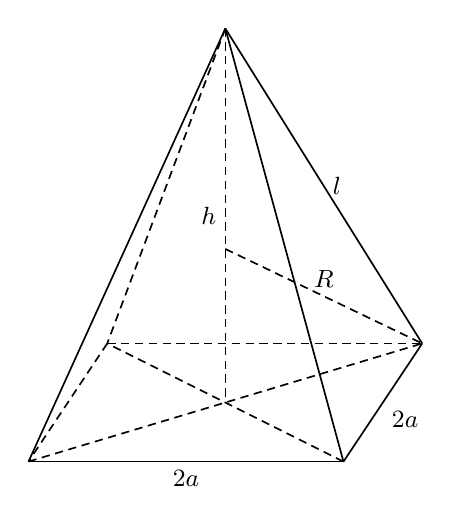
\begin{tikzpicture}[line width=.6pt, font=\small]
\coordinate (S) at (0.5,4.5);
\coordinate (VFL) at (-2,-1);
\coordinate (VFR) at (2,-1);
\coordinate (VBR) at (3,0.5);
\coordinate (VBL) at (-1,0.5);
\coordinate (O0) at (0.5,-0.25);
\coordinate (Q) at (0.5000000000,1.7000000000);
% base front solid
\draw (VFL)--(VFR) node[midway,below=2pt,inner sep=1pt] {$2a$};
\draw (VFR)--(VBR) node[midway,below right=2pt,inner sep=1pt] {$2a$};

% base back dashed
\draw[densely dashed] (VBL)--(VBR);
\draw[densely dashed] (VBL)--(VFL);
% base diagonals dashed
\draw[densely dashed] (VFL)--(VBR);
\draw[densely dashed] (VFR)--(VBL);
% laterals
\draw (S)--(VFL);
\draw (S)--(VFR);
\draw (S)--(VBR) node[midway,right=2pt,inner sep=1pt] {$l$};
\draw[densely dashed] (S)--(VBL);
% height
\draw[densely dashed] (S)--(O0) node[midway,left=2pt,inner sep=1pt] {$h$};
% sphere radius horizontal
\draw[densely dashed] (Q)--(VBR) node[midway,above=2pt,inner sep=1pt] {$R$};
\end{tikzpicture}
